\documentclass[12pt]{article}
% Full article preamble (duplicated, no common file)
\usepackage{fontspec}
\usepackage[a4paper,margin=2.5cm,includefoot]{geometry}
\usepackage{polyglossia}
\usepackage{amsmath}
\usepackage{amssymb}
\usepackage{xcolor}
\usepackage{fancyhdr}
\usepackage{graphicx}
\usepackage{listings}
\usepackage[most]{tcolorbox}
\usepackage{pifont}
\usepackage{enumitem}
\usepackage{titlesec}
\usepackage[bottom]{footmisc}
\usepackage{titling}
\usepackage{minted}
\usepackage{etoolbox}
\usepackage{array}
\usepackage{extsizes}

\newfontfamily\emoji{Segoe UI Emoji}

\pagestyle{fancy}

\setmainlanguage[numerals=western]{arabic}
\setotherlanguage{english}
\newfontfamily\arabicfont[Script=Arabic]{Amiri}
\newfontfamily\arabicfonttt[Script=Arabic]{Courier New}

\lstset{
  language=[Sharp]C,
  numbers=left,
  stepnumber=1,
  numbersep=8pt,
  frame=single,
  basicstyle=\ttfamily\small,
  keywordstyle=\color{blue},
  stringstyle=\color{red},
  commentstyle=\color{green!50!black}
}

\newif\ifdetailed
\ifdefined\setdetailed
  \setdetailed
\fi

\newif\ifwithsols
\ifdefined\setwithsols
  \setwithsols
\fi

% unified tcolorboxes for articles
\tcbset{colback=white, colframe=black, fonttitle=\bfseries, boxrule=0.8pt}
\newtcolorbox{boxDef}[1][]{colback=blue!5!white,colframe=blue!75!black,
  title={{\emoji📘} تعريف\ifx\\#1\\\else ~#1\fi :}}
\newtcolorbox{boxExercise}[1][]{colback=cyan!5!white,colframe=cyan!70!black,
  title={{\emoji🧩} تمرين\ifx\\#1\\\else ~#1\fi :}}
\newtcolorbox{boxExample}[1][]{colback=yellow!5!white,colframe=orange!90!black,
  title={{\emoji📝} مثال\ifx\\#1\\\else ~#1\fi :}}
\newtcolorbox{boxNote}[1][]{colback=gray!10!white,colframe=black,
  title={{\emoji✨} ملاحظة\ifx\\#1\\\else ~#1\fi :}}
\newtcolorbox{boxAttention}[1][]{colback=magenta!10!white,colframe=magenta!80!black,
  title={{\emoji🔔} تنبيه\ifx\\#1\\\else ~#1\fi :}}
\newtcolorbox{boxWarning}[1][]{colback=red!5!white,colframe=red!75!black,
  title={{\emoji⚡} ملاحظة هامة\ifx\\#1\\\else ~#1\fi :}}
\newtcolorbox{boxSolution}[1][]{colback=green!5!white,colframe=green!60!black,
  title={{\emoji✅} حل\ifx\\#1\\\else ~#1\fi :}}
\newtcolorbox{boxSymbol}[1][]{colback=purple!5!white,colframe=purple!70!black,
  title={{\emoji🔣} رمز\ifx\\#1\\\else ~#1\fi :}}

\tcbset{simplecode/.style={ colback=gray!5, colframe=black!50, boxrule=0.4pt, arc=2pt, left=4pt,right=4pt,top=4pt,bottom=4pt}}
\newenvironment{boxCode}{\begin{tcolorbox}[simplecode]}{\end{tcolorbox}}

\newcolumntype{C}[1]{>{\centering\arraybackslash}p{#1}}

% redefine spaces after titles
\makeatletter
\renewcommand{\@maketitle}{%
  \begin{center}
    {\huge \bfseries \@title \par}%
    \vskip 0.2em % space between title and author
    {\large \@author \par}%
    % \vskip 0.2em % space between author and date
    % {\normalsize \@date \par}%
  \end{center}
}
\makeatother

\fancyhf{} % clear default
\fancypagestyle{plain}{
  \fancyhf{}
  \fancyhead[L]{مدرسة التسامح الشاملة}
  % \fancyhead[L]{
\includegraphics[height=1cm]{../../../images/logoTasamoh.png}}
  \fancyhead[R]{الأستاذ محمود اغبارية}
  \fancyfoot[C]{\thepage}
}

\fancyhead[L]{مدرسة التسامح الشاملة}
\fancyhead[R]{الأستاذ محمود اغبارية}
\fancyfoot[C]{\thepage}
% \date{\today}

\setcounter{tocdepth}{3} % only section subsection and subsubsection in TOC


% ----------------------


% \begin{document}

% \maketitle

% % \clearpage  % start TOC on a new page
% % \renewcommand{\contentsname}{جدول المحتويات}
% % \tableofcontents
% % \clearpage

% \part*{part 1} % the * prevents numbering
% \section*{مقدمة}
% \subsection*{مثال رياضي}
% \subsubsection*{مثال فرعي}
% \paragraph*{ paragraph 1}
% \subparagraph*{sub paragraph 1}

% \ifdetailed
% \begin{english}
% \begin{minted}{csharp}
% // C# Example
% \end{minted}
% \end{english}
% \fi

% OLD WAY
% \ifdetailed
% \begin{english}
% \begin{lstlisting}
% // C# Example
% \end{lstlisting}
% \end{english}
% \fi

% % 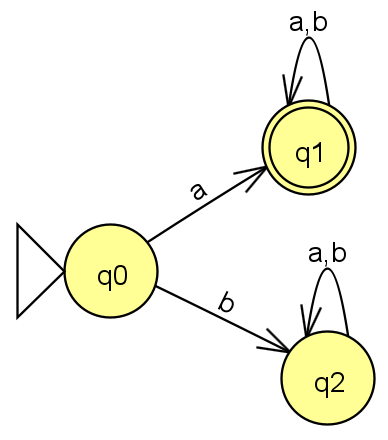
\includegraphics[width=0.2\textwidth]{../../../images/DFAs/ex1_q1.png}



% \vspace{3cm}
% \begin{flushleft}
% أرجو لكم وقتًا ممتعًا.

% الأستاذ محمود اغبارية.
% \end{flushleft}


% \end{document}


\title{ورقة تمرن 3 للصف العاشر 10 $\mathtt{Math\ Library}$}

\begin{document}

\maketitle
\thispagestyle{fancy}


\begin{enumerate}[itemsep=3em]

    \item
    اكتب برنامجا يستقبل من المستخدم رقمين، ثم يطبع تربيع الرقم الصغير وجذر الرقم الكبير.
    \ifdetailed
    \begin{boxExample}
    \begin{english}
    \begin{minted}{csharp}
Please enter 2 numbers:
4
9
The sqrt of the max = 3
The square of the min = 16
    \end{minted}
    \end{english}
    \end{boxExample}
    \ifwithsols
    \begin{boxSolution}
    \begin{english}
    \begin{minted}{csharp}
int n1 = int.Parse(Console.ReadLine());
int n2 = int.Parse(Console.ReadLine());
int max = Math.Max(n1, n2);
int min = Math.Min(n1, n2);
Console.WriteLine("The sqrt of the max = " + Math.Sqrt(max));
Console.WriteLine("The square of the min = " + Math.Pow(min, 2));
    \end{minted}
    \end{english}
    \end{boxSolution}
    \clearpage
    \fi
\fi

    \item
    اكتب برنامجًا يقرأ عددين صحيحين من المستخدم، ويطبع الفرق المطلق بينهما (الفرق بينهما بالقيمة المطلقة).
    \ifdetailed
    \begin{boxExample}
    \begin{english}
    \begin{minted}{csharp}
Please enter 2 numbers:
5
12
The absolute difference = 7
    \end{minted}
    \end{english}
    \end{boxExample}
    \ifwithsols
    \begin{boxSolution}[1]
    \begin{english}
    \begin{minted}{csharp}
int a = int.Parse(Console.ReadLine());
int b = int.Parse(Console.ReadLine());
int diff = Math.Abs(a - b);
Console.WriteLine("The absolute difference = " + diff);
    \end{minted}
    \end{english}
    \end{boxSolution}
    \begin{boxSolution}[2]
    \begin{english}
    \begin{minted}{csharp}
int a = int.Parse(Console.ReadLine());
int b = int.Parse(Console.ReadLine());
int max = Math.Max(a, b);
int min = Math.Min(a, b);
Console.WriteLine("The absolute difference = " + (max - min));
    \end{minted}
    \end{english}
    \end{boxSolution}
    \fi
    \clearpage
\fi

    \item
    اكتب برنامجًا يقرأ إحداثيات نقطتين في المستوى (أي يقرأ 4 أرقام) $(x_1, y_1)$ و $(x_2, y_2)$،
    ثم يحسب المسافة بينهما باستخدام:
    $$d = \sqrt{(x_2 - x_1)^2 + (y_2 - y_1)^2}$$
    \ifdetailed
    \begin{boxExample}
    \begin{english}
    \begin{minted}{csharp}
Please enter x1, y1, x2, y2:
0
0
3
4
Distance = 5
    \end{minted}
    \end{english}
    \end{boxExample}
    \ifwithsols
    \begin{boxSolution}
    \begin{english}
    \begin{minted}{csharp}
int x1 = int.Parse(Console.ReadLine());
int y1 = int.Parse(Console.ReadLine());
int x2 = int.Parse(Console.ReadLine());
int y2 = int.Parse(Console.ReadLine());
double diffx = Math.Pow(x2 - x1, 2);
double diffy = Math.Pow(y2 - y1, 2);
double d = Math.Sqrt(diffx + diffy);
Console.WriteLine("Distance = " + d);
    \end{minted}
    \end{english}
    \end{boxSolution}
    \clearpage
    \fi
\fi

    \item
    اكتب برنامجًا يقرأ ثلاثة أعداد من المستخدم، ويطبع الأكبر بينها.
    \ifdetailed
    \begin{boxExample}
    \begin{english}
    \begin{minted}{csharp}
Please enter 3 numbers:
5
12
7
The maximum = 12
    \end{minted}
    \end{english}
    \end{boxExample}
    \ifwithsols
    \begin{boxSolution}
    \begin{english}
    \begin{minted}{csharp}
int a = int.Parse(Console.ReadLine());
int b = int.Parse(Console.ReadLine());
int c = int.Parse(Console.ReadLine());
int max = Math.Max(a, b);
max = Math.Max(max, c);
Console.WriteLine("The maximum = " + max);
    \end{minted}
    \end{english}
    \end{boxSolution}
    \fi
\fi

    \item
    اكتب برنامجًا يقرأ أربعة أعداد من المستخدم ويطبع الأصغر بينها.
    \ifdetailed
    \begin{boxExample}
    \begin{english}
    \begin{minted}{csharp}
Please enter 4 numbers:
8
3
15
6
The minimum = 3
    \end{minted}
    \end{english}
    \end{boxExample}
    \ifwithsols
    \begin{boxSolution}
    \begin{english}
    \begin{minted}{csharp}
int a = int.Parse(Console.ReadLine());
int b = int.Parse(Console.ReadLine());
int c = int.Parse(Console.ReadLine());
int d = int.Parse(Console.ReadLine());
int min1 = Math.Min(a, b);
int min2 = Math.Min(c, d);
int min = Math.Min(min1, min2);
Console.WriteLine("The minimum = " + min);
    \end{minted}
    \end{english}
    \end{boxSolution}
    \fi
    \clearpage
\fi

    \item
    اكتب برنامجًا يستقبل ثلاثة أعداد، ويطبع الفرق الأكبر بين رقمين من بين الثلاثة.
    \ifdetailed
    \begin{boxExample}
    \begin{english}
    \begin{minted}{csharp}
Please enter 3 numbers:
10
3
20
The largest difference = 17
    \end{minted}
    \end{english}
    \end{boxExample}
    \ifwithsols
    \begin{boxSolution}[1]
    \begin{english}
    \begin{minted}{csharp}
int a = int.Parse(Console.ReadLine());
int b = int.Parse(Console.ReadLine());
int c = int.Parse(Console.ReadLine());
int max = Math.Max(a, Math.Max(b, c));
int min = Math.Min(a, Math.Min(b, c));
int diff = max - min;
Console.WriteLine("The largest difference = " + diff);
    \end{minted}
    \end{english}
    \end{boxSolution}
    \begin{boxSolution}[2]
    \begin{english}
    \begin{minted}{csharp}
int a = int.Parse(Console.ReadLine());
int b = int.Parse(Console.ReadLine());
int c = int.Parse(Console.ReadLine());
int diff1 = Math.Abs(a-b);
int diff2 = Math.Abs(a-c);
int diff3 = Math.Abs(b-c);
int maxDiff = Math.Max(diff1, Math.Max(diff2, diff3));
Console.WriteLine("The largest difference = " + maxDiff);
    \end{minted}
    \end{english}
    \end{boxSolution}
    \clearpage
    \fi
\fi

    \item
    اكتب برنامجًا يقرأ عددًا عشريًا من المستخدم (مثلاً 12.34567) ويقرّبه إلى منزلتين عشريتين فقط.
    \ifdetailed
    \begin{boxExample}
    \begin{english}
    \begin{minted}{csharp}
Please enter a decimal number:
12.34567
Rounded to 2 decimals = 12.35
    \end{minted}
    \end{english}
    \end{boxExample}
    \ifwithsols
    \begin{boxSolution}
    \begin{english}
    \begin{minted}{csharp}
double n = double.Parse(Console.ReadLine());
n = n * 100;
double rounded = Math.Round(n);
rounded = rounded / 100;
Console.WriteLine("Rounded to 2 decimals = " + rounded);
    \end{minted}
    \end{english}
    \end{boxSolution}
    \fi
    \fi

    \item
    اكتب برنامجًا يقرأ عددًا صحيحًا موجبًا من المستخدم، ثم يحسب أكبر عدد صحيح $n$ بحيث:
    $$ n^2 \leq \text{العدد} $$
    \ifdetailed
    \begin{boxExample}
    \begin{english}
    \begin{minted}{csharp}
Please enter a positive integer:
20
The largest n with n^2 <= number is 4
    \end{minted}
    \end{english}
    \end{boxExample}
    \ifwithsols
    \begin{boxSolution}
    \begin{english}
    \begin{minted}{csharp}
int num = int.Parse(Console.ReadLine());
int n = (int) Math.Sqrt(num);
Console.WriteLine("The largest n with n^2 <= number is " + n);
    \end{minted}
    \end{english}
    \end{boxSolution}
    \fi
\fi
\end{enumerate}

\end{document}
